%导演区
\documentclass[a4paper,11pt,UTF8]{article}%book,report,letter
\usepackage[table]{xcolor}
\usepackage{ctex}
\usepackage{geometry}
\geometry{a4paper,scale=0.8}
\usepackage{amsfonts}
\usepackage{amssymb}
\usepackage{verbatim}
\usepackage{mathrsfs}
\usepackage[arrow,matrix]{xy}
\usepackage{amsmath,amssymb,amscd,bm,bbm,amsthm,mathrsfs}
\usepackage{amsmath,amscd}
\usepackage{amsfonts,amssymb}
\usepackage{xypic}
\usepackage{indentfirst}
\usepackage{diagbox}
\usepackage{graphicx}
\usepackage{subfig}    %% 子图包
\usepackage{float} 
\usepackage{caption}
\captionsetup{labelfont=bf}
\usepackage{zhnumber} % change section number to chinese
%这下面为在latex中插入代码所需环境
\usepackage{CJK}
\usepackage{listings}
\usepackage{xcolor}
\lstset{
	language=Matlab,  %代码语言使用的是matlab
	frame=shadowbox, %把代码用带有阴影的框圈起来
	rulesepcolor=\color{red!20!green!20!blue!20},%代码块边框为淡青色
	keywordstyle=\color{blue!90}\bfseries, %代码关键字的颜色为蓝色,粗体
	commentstyle=\color{red!10!green!70}\textit,    % 设置代码注释的颜色
	showstringspaces=false,%不显示代码字符串中间的空格标记
	numbers=left, % 显示行号
	numberstyle=\tiny,    % 行号字体
	stringstyle=\ttfamily, % 代码字符串的特殊格式
	breaklines=true, %对过长的代码自动换行
	extendedchars=false,  %解决代码跨页时,章节标题,页眉等汉字不显示的问题
	texcl=true}
\def\d{\textup{d}}

\theoremstyle{plain}
\newtheorem{thm}{定理}[section]
\newtheorem{lem}{引理}[section]
\newtheorem{prop}{命题}[section]
\newtheorem{cor}{推论}[section]


\renewcommand{\qedsymbol}{$\square$}
\renewcommand\baselinestretch{1.25}
\renewcommand\thesection{\zhnum{section}}
\renewcommand \thesubsection {\arabic{section}}

\usepackage{tabu}                     % 表格插入
\usepackage{multirow}                 % 一般用以设计表格,将所行合并
\usepackage{multicol}                 % 合并多列
\usepackage{multirow}                % 合并多行
\usepackage{float}                    % 图片浮动
\usepackage{makecell}                 % 三线表-竖线
\usepackage{booktabs} 
%正文区
\begin{document}
	\title{\heiti 课题组组会-练习5}
	\author{王程 }
	\date{\today}
	\maketitle
	
	\section{练习及结果}
	1.在$x\in \left[0,1\right]$的均匀网格上尝试使用 Hybrid Least Squares Reconstruction(HLSr) 对$f\left(x\right)$ 及$g\left(x\right)$进行Hyperbolic rDG的DG(P0P3)+rDG(P1P2) 重构,其中$f\left(x\right)=1+x+x^2+x^3, g\left(x\right)=sin\left(\pi x\right)$.\\
	\indent a)写出对于第i个单元的重构超定方程组,并测试重构精度。\\
	\indent b)如果网格为不均匀网格呢?\\
	~\\
	\indent 2.在$x\in \left[0,1\right]$ 的均匀网格上尝试使用 Variational Reconstruction(VR) 对$f\left(x\right),g\left(x\right)$ 进行P0P1重构,其中$f\left(x\right)=1+x, g\left(x\right)=sin\left(\pi x\right)$\\
	\indent a)尝试调整不同阶次的权重系数及边界面权重系数,测试重构精度。\\
	\indent b)如果为不均匀网格呢?\\
	
	\noindent \textbf{解:1.}\\
	\indent 本题均考虑非均匀网格,均匀网格视为非均匀网格的特例。\\
	\indent 第i个单元的重构超定方程组为:\\
	$$\left\{
	\begin{aligned}
	\int_{\Omega_{i+1}}\varphi^R_id\Omega&=\int_{\Omega_{i+1}}\varphi_{i+1}d\Omega	\\
	\int_{\Omega_{i+1}}v^R_id\Omega&=\int_{\Omega_{i+1}}v_{i+1}d\Omega\\
	\frac{\partial v^R_i}{\partial x}|_{x^{i+1}_c}&=\frac{\partial v_{i+1}}{\partial x}|_{x^{i+1}_c}		
	\end{aligned}
	\right.$$\\
	将其转化成$Ax=b$的形式,
	\begin{equation*}
	\begin{pmatrix}
		\frac{\overline{B^i_4}}{\Delta x_{i+1}}\\
		~\\
		\frac{\overline{B^i_3}}{\Delta x_{i+1}\Delta x_{i}}\\
		~\\
		\frac{\left(x^{i+1}_c-x^i_c\right)^2\Delta x^2_{i+1}}{\Delta x^3_i}
	\end{pmatrix}
	\begin{pmatrix}
	\varphi^{c,R}_{xxx}\Delta x^3_i\\
	~\\
	\varphi^{c,R}_{xxx}\Delta x^3_i\\
	~\\
	\varphi^{c,R}_{xxx}\Delta x^3_i
\end{pmatrix}=
	\begin{pmatrix}
	\overline{\varphi_{i+1}}-\overline{\varphi_i}-\overline{\varphi^i_x}\Delta x_i \frac{x^{i+1}_c-x^i_c}{\Delta x_i}-\varphi^{c,i}_{xx}\Delta x^2_i \frac{\overline{B^i_3}}{\Delta x_{i+1}}\\
	~\\
	\overline{\varphi^{i+1}_x}-\overline{\varphi^i_x}\Delta x_i \Delta x^{-1}_i-\varphi^c_{xx}\Delta x^2_i \frac{x^{i+1}_c-x^i_c}{\Delta x^2_i}\\
	~\\
	\varphi^{c,i+1}_{xx}\Delta x^2_{i+1}-\varphi^c_{xx}\Delta x^2_i\frac{\Delta x^2_{i+1}}{\Delta x^2_i}
\end{pmatrix}
\end{equation*}	\\
最终得到$f\left(x\right)$与$g\left(x\right)$的重构比较图以及精度分析图:\\
	\begin{figure}[!h]
	\centering
	\subfloat[f重构]{
		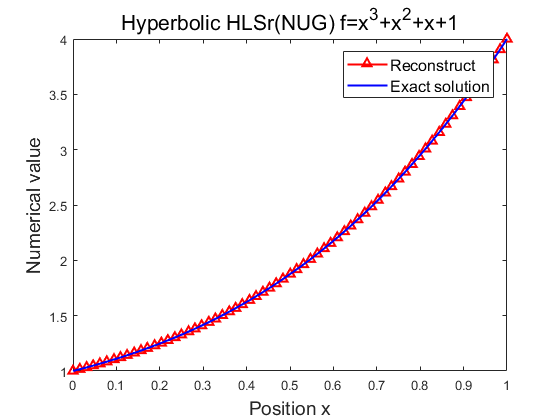
\includegraphics[width=3in]{HLSr/fu64.png} 
	}
	\hfill
	\subfloat[g重构]{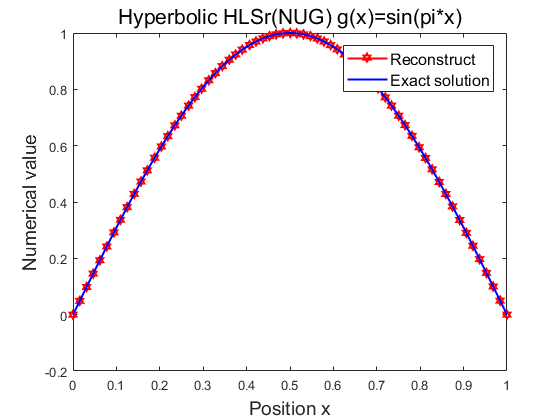
\includegraphics[width=3in]{HLSr/gu64.png} }
	\caption{Hyperbolic HLSr DG(P0P3)+rDG(P1P2)}
\end{figure}\\

	\begin{figure}[!h]
	\centering
	\subfloat[f精度分析]{
		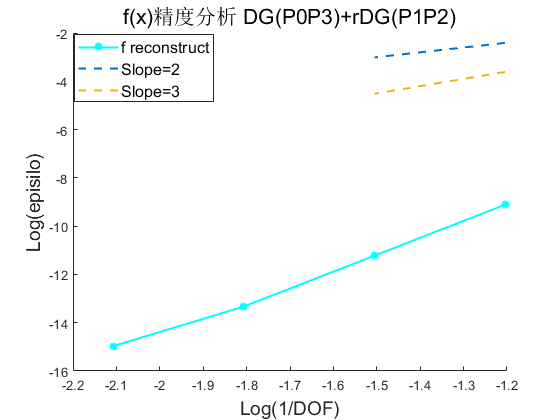
\includegraphics[width=3in]{HLSr/f精度分析.png} 
	}
	\hfill
	\subfloat[g精度分析]{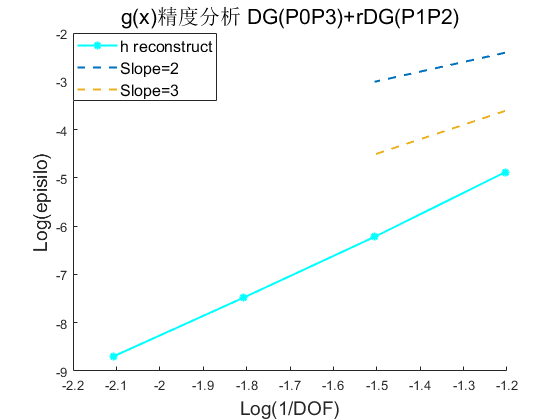
\includegraphics[width=3in]{HLSr/h精度分析.png} }
	\caption{精度分析-单元格数为8,16,32,64}
\end{figure}
\clearpage
 \noindent 注:若对f考虑单元格数为64,128,256,512的精度分析,则可达到机器误差\\
	\begin{figure}[!h]
	\centering
	{
		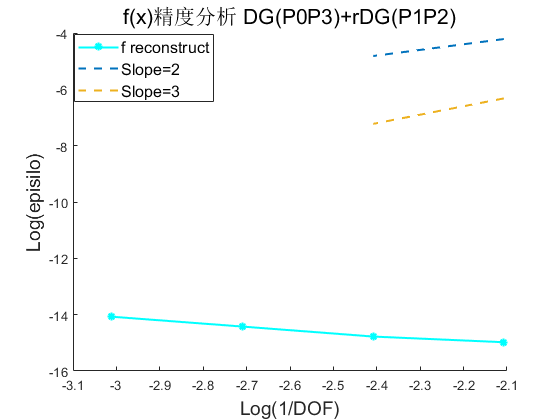
\includegraphics[width=3in]{HLSr/f精度分析64.png} 
	}
	\caption{精度分析-单元格数为64,128,256,512}
\end{figure}\\
\noindent \textbf{解:2.}\\
\indent 本题均考虑非均匀网格,均匀网格视为非均匀网格的特例。\\
\indent 设置权重系数$\omega_0=1,\omega_1=0.5,\omega_b=1$, 对$f\left(x\right)=1+x$和$g\left(x\right)=sin\left(\pi x\right)$进行VR重构,以下给出Nelem=8时候的重构图:\\
\begin{figure}[!h]
	\centering
	\subfloat[f重构]{
		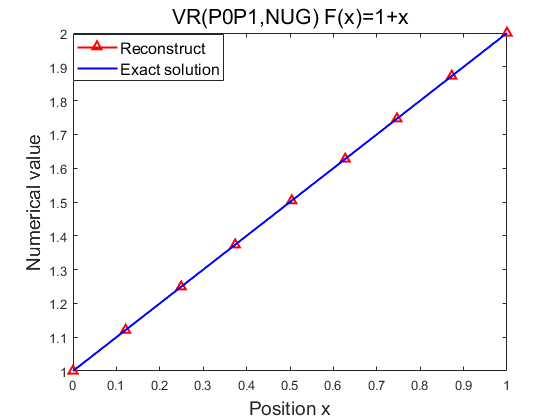
\includegraphics[width=3in]{VR/fu8.png} 
	}
	\hfill
	\subfloat[g重构]{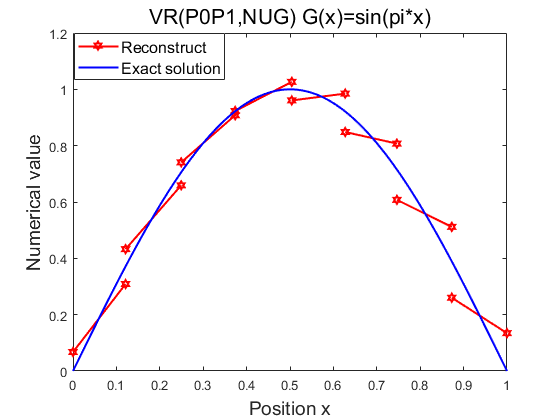
\includegraphics[width=3in]{VR/gu8.png} }
	\caption{VR重构(Nelem=8) }
\end{figure}
并对该情况下的$f,g$进行精度分析:\\
\clearpage
\begin{figure}[!h]
	\centering
	\subfloat[f精度分析]{
		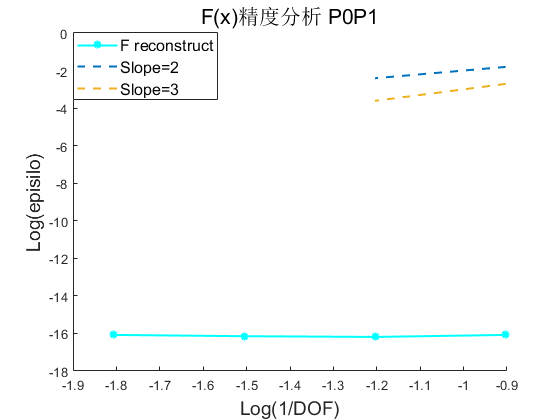
\includegraphics[width=3in]{VR/F1-0.5-1.png} 
	}
	\hfill
	\subfloat[g精度分析]{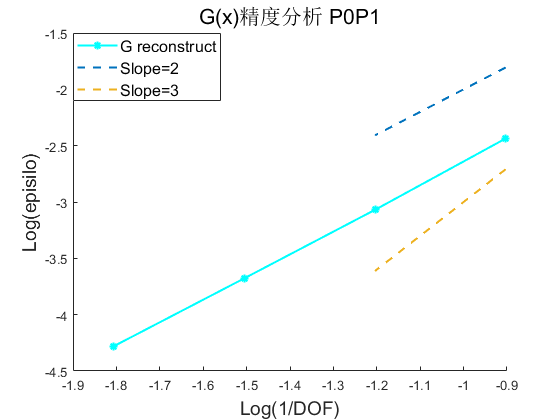
\includegraphics[width=3in]{VR/G1-0.5-1.png} }
	\caption{VR精度分析}
\end{figure}
\noindent 调整权重系数以及边界面权重系数,测试重构精度,得到以下结论:\\
~\\
\begin{comment}

\textbf{对$G\left(x\right)=sin\left(\pi x\right)$而言:}\\
\indent $\omega_0$与$\omega_1$其中之一为0,精度很差\\
\indent $\omega_0$与$\omega_1$固定,$\omega_b$$\uparrow 1$,精度表现$\uparrow$\\
\indent $\omega_0$与$\omega_b$固定,$\omega_1$$\downarrow 0.25$,精度表现$\uparrow$\\
\indent $\omega_1$与$\omega_b$固定,$\omega_0$$\uparrow 1$,精度表现$\uparrow$\\
~\\
\textbf{对$F\left(x\right)=1+x$而言:}\\
\indent $\omega_0$与$\omega_1$其中之一为0,精度很差\\
\indent $\omega_0$与$\omega_1$固定,$\omega_b$$\uparrow 1$,精度表现$\uparrow$\\
\indent $\omega_0$与$\omega_b$固定,$\omega_1$$\uparrow 0.5$,精度表现$\uparrow$\\
\indent $\omega_1$与$\omega_b$固定,$\omega_0$$\downarrow 0.5$,精度表现$\uparrow$\\
~\\
\end{comment}


\begin{minipage}[c]{0.5\textwidth}
	\centering
\label{tbl:table1}
\captionof{table}{$G\left(x\right)$精度与$\omega_0$,$\omega_1$,$\omega_b$的关系} 
\begin{tabular}{ccccc}
	\Xhline{2pt}
	\multirow{2}{*}{$\omega_0$} & \multirow{2}{*}{$\omega_1$}& \multirow{2}{*}{$\omega_b$} & \multirow{2}{*}{精度表现}  \\
	\\
	\Xhline{0.5pt}\\
	0&—&—&差\\
	\Xhline{0.5pt}\\
	—&0&—&差\\
	\Xhline{0.5pt}\\
	—&—& $\uparrow 1$&$\uparrow$ \\
	\Xhline{0.5pt}\\
	—&$\downarrow 0.25$&—&$\uparrow$\\
	\Xhline{0.5pt}\\
	$\uparrow 1$&—&—&$\uparrow$\\         
	\Xhline{2pt}
\end{tabular}
\end{minipage}
\begin{minipage}[c]{0.5\textwidth}
	\centering
	\label{tbl:table1}
	\captionof{table}{$F\left(x\right)$精度与$\omega_0$,$\omega_1$,$\omega_b$的关系}  
	\begin{tabular}{ccccc}
		\Xhline{2pt}
		\multirow{2}{*}{$\omega_0$} & \multirow{2}{*}{$\omega_1$}& \multirow{2}{*}{$\omega_b$} & \multirow{2}{*}{精度表现}  \\
		\\
		\Xhline{0.5pt}\\
		0&—&—&差\\
		\Xhline{0.5pt}\\
		—&0&—&差\\
		\Xhline{0.5pt}\\
		—&—& $\uparrow 1$&$\uparrow$ \\
		\Xhline{0.5pt}\\
		—&$\uparrow 0.5$&—&$\uparrow$\\
		\Xhline{0.5pt}\\
		$\downarrow 0.5$&—&—&$\uparrow$\\         
		\Xhline{2pt}
	\end{tabular}
\end{minipage}\\
~\\


下面给出部分精度分析图:
\begin{figure}[!h]
	\centering
	\subfloat[$\omega_0=1,\omega_1=0.5,\omega_b=0$]{
		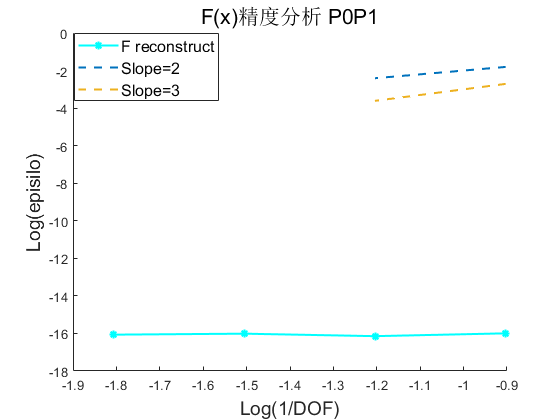
\includegraphics[width=2.5in]{VR/F1-0.5-0.png} 
	}
	\hfill
	\subfloat[$\omega_0=1,\omega_1=0.5,\omega_b=0$]{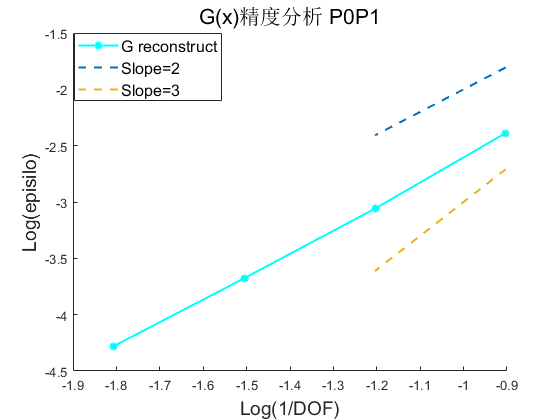
\includegraphics[width=2.5in]{VR/G1-0.5-0.png} }\\
		\subfloat[$\omega_0=1,\omega_1=0,\omega_b=0$]{
		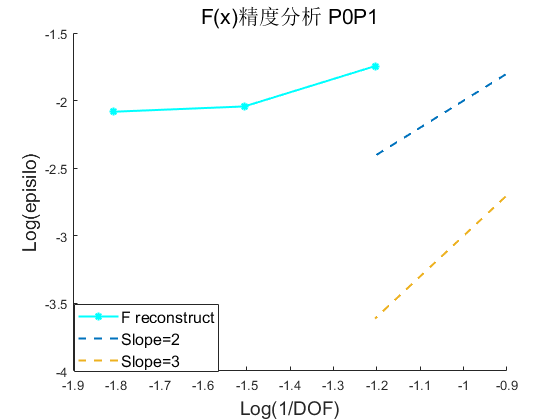
\includegraphics[width=2.5in]{VR/F1-0-0.png} 
	}
	\hfill
	\subfloat[$\omega_0=1,\omega_1=0,\omega_b=0$]{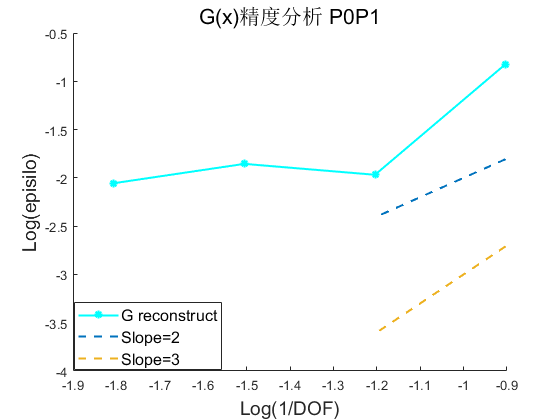
\includegraphics[width=2.5in]{VR/G1-0-0.png} }\\
	\subfloat[$\omega_0=0,\omega_1=1,\omega_b=0$]{
		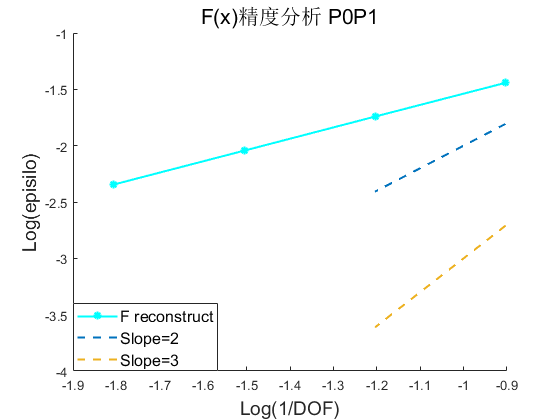
\includegraphics[width=2.5in]{VR/F0-1-0.png} 
	}
	\hfill
	\subfloat[$\omega_0=0,\omega_1=1,\omega_b=0$]{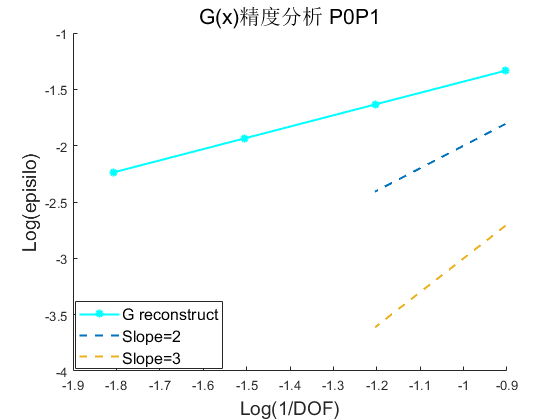
\includegraphics[width=2.5in]{VR/G0-1-0.png} }\\
	\subfloat[$\omega_0=0.5,\omega_1=0.5,\omega_b=0$]{
		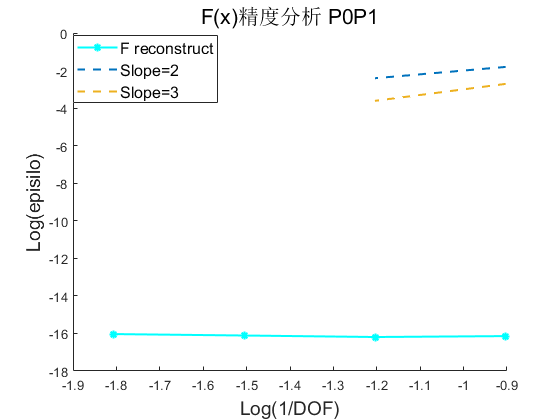
\includegraphics[width=2.5in]{VR/F0.5-0.5-0.png} 
	}
	\hfill
	\subfloat[$\omega_0=0.5,\omega_1=0.5,\omega_b=0$]{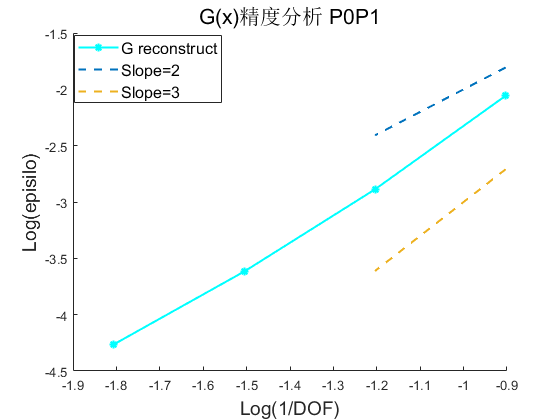
\includegraphics[width=2.5in]{VR/G0.5-0.5-0.png} }
	
	
	
	
	\caption{VR精度分析(调整权重系数)}
\end{figure}



	\clearpage
	\section{附录(代码,仅展示部分)}
	\noindent \textbf{VR}
	\lstset{language=Matlab}%代码语言使用的是matlab
	\lstset{breaklines}%自动将长的代码行换行排版
	\lstset{extendedchars=false}%解决代码跨页时,章节标题,页眉等汉字不显示的问题
\begin{lstlisting}
clc
clear all
close all
%% Pre-proceeding
Unit=8;endx=1;deltax=endx/Unit;numberx=Unit+1;omega0=1;omega1=0.5;omegab=1;
%记录内点位置,上下浮动不超过百分之5
Grid=zeros(1,numberx);
Deltax=zeros(1,Unit);
for i=2:numberx-1
Grid(1,i)=(i-1)*deltax+(0.1*rand(1)-0.05)*deltax;
end
Grid(1,numberx)=endx;
for i=2:numberx
Deltax(i-1)=Grid(1,i)-Grid(1,i-1);%记录每个单元的区间长度
end
f=@(x)1+x;F=@(x)1;
h=@(x)sin(pi*x);H=@(x)pi*cos(pi*x);
Unumsolution=zeros(1,Unit);
Ureconstruct=zeros(Unit,1);
A=sparse(1:Unit,1:Unit,0,Unit,Unit);
R=zeros(Unit,1);
Unumsolution1=zeros(1,2);
Unumsolution2=zeros(2,numberx-1);
Acc=zeros(3,4);a1=[1/8,1/16,1/32,1/64];a2=[1/8,1/16];

%% Proceeding
%对f
%initial 
for i=1:numberx-1
Unumsolution(1,i)=1+0.5*(Grid(i+1)+Grid(i));
end

%构建大型稀疏矩阵
for iface=2:numberx-1
ieL=iface-1;xciL=0.5*(Grid(ieL)+Grid(ieL+1));
ieR=iface;xciR=0.5*(Grid(ieR)+Grid(ieR+1));
dLR=0.5*(Deltax(ieR)+Deltax(ieL));
A(ieL,ieL)=A(ieL,ieL)+2*(omega0^2*((Grid(iface)-xciL)/Deltax(ieL))^2+omega1^2*dLR^2/Deltax(ieL)^2)/dLR;
A(ieL,ieL+1)=A(ieL,ieL+1)-2*(omega0^2*((Grid(iface)-xciL)/Deltax(ieL))*((Grid(iface)-xciR)/Deltax(ieR))+omega1^2*dLR^2/(Deltax(ieR)*Deltax(ieL)))/dLR;
R(ieL)=R(ieL)-2*omega0^2*(Unumsolution(ieL)-Unumsolution(ieR))*((Grid(iface)-xciL)/Deltax(ieL))/dLR;

A(ieR,ieR)=A(ieR,ieR)+2*(omega0^2*((Grid(iface)-xciR)/Deltax(ieR))^2+omega1^2*dLR^2/Deltax(ieR)^2)/dLR;
A(ieR,ieR-1)=A(ieR,ieR-1)-2*(omega0^2*((Grid(iface)-xciL)/Deltax(ieL))*((Grid(iface)-xciR)/Deltax(ieR))+omega1^2*dLR^2/(Deltax(ieR)*Deltax(ieL)))/dLR;
R(ieR)=R(ieR)+2*omega0^2*(Unumsolution(ieL)-Unumsolution(ieR))*((Grid(iface)-xciR)/Deltax(ieR))/dLR;
end

%B.C
%left
iface=1;
ieR=iface;
xciR=0.5*(Grid(ieR)+Grid(ieR+1));
A(ieR,ieR)=A(ieR,ieR)+4*omegab^2*((Grid(iface)-xciR)/Deltax(ieR))^2/Deltax(ieR);
R(ieR)=R(ieR)+4*omegab^2*(1-Unumsolution(ieR))*((Grid(iface)-xciR)/Deltax(ieR))/Deltax(ieR);

%Right
iface=numberx;
ieL=iface-1;
xciL=0.5*(Grid(ieL)+Grid(ieL+1));
A(ieL,ieL)=A(ieL,ieL)+4*omegab^2*((Grid(iface)-xciL)/Deltax(ieL))^2/Deltax(ieL);
R(ieL)=R(ieL)+4*omegab^2*(2-Unumsolution(ieL))*((Grid(iface)-xciL)/Deltax(ieL))/Deltax(ieL);


%Thomas 解三对角矩阵
L=zeros(1,Unit);U=zeros(1,Unit);C=zeros(1,Unit);
U(1)=A(1,1);
for i=2:numberx-1
L(i)=A(i,i-1)/U(i-1);
U(i)=A(i,i)-L(i)*A(i-1,i);
end
Y=zeros(Unit,1);
Y(1)=R(1);
for i=2:numberx-1
Y(i)=R(i)-L(i)*Y(i-1);
end
Ureconstruct(numberx-1)=Y(numberx-1)/U(numberx-1);
for i=numberx-2:-1:1
Ureconstruct(i)=(Y(i)-A(i,i+1)*Ureconstruct(i+1))/U(i);
end





%% Post-proceeding
figure
k=1;
x=Grid(k):1*(Grid(k+1)-Grid(k)):Grid(k+1);
xci=(Grid(k+1)+Grid(k))/2;
p=@(x)Unumsolution(1,k)+Ureconstruct(k,1)*(x-xci)/Deltax(k);
y=p(x);
plot(x,y,'-r^','linewidth',1.5);hold on
H1=plot(x,y,'-r^','linewidth',1.5);hold on

for k=2:numberx-1
x=Grid(k):1*(Grid(k+1)-Grid(k)):Grid(k+1);
xci=(Grid(k+1)+Grid(k))/2;
p=@(x)Unumsolution(1,k)+Ureconstruct(k,1)*(x-xci)/Deltax(k);
y=p(x);
plot(x,y,'-r^','linewidth',1.5);
end

hold on
x=Grid(1):0.01*(Grid(numberx)-Grid(1)):Grid(numberx);
plot(x,f(x),'-b','linewidth',1.5);
H2=plot(x,f(x),'-b','linewidth',1.5);
lgd=legend([H1,H2],'Reconstruct','Exact solution');
lgd.FontSize=12;
xlabel('Position x','fontsize',14)
ylabel('Numerical value','fontsize',14)
title('VR(P0P1,NUG) F(x)=1+x','fontsize',16)
hold off

%计算精度
Acc(1,1)=Accuracy(8);
Acc(1,2)=Accuracy(16);
Acc(1,3)=Accuracy(32);
Acc(1,4)=Accuracy(64);
for k=1:3
accuracyf(k)=(log10(Acc(1,k+1))-log10(Acc(1,k)))./(log10(a1(1,k+1))-log10(a1(1,k)));
end

figure
hold on
plot(log10(a1),log10(Acc(1,:)),'-c*','linewidth',1.5)
H1=plot(log10(a1),log10(Acc(1,:)),'-c*','linewidth',1.5);

H2=plot(log10(a2),2*log10(a2),'--','linewidth',1.5);
plot(log10(a2),3*log10(a2),'--','linewidth',1.5)
H3=plot(log10(a2),3*log10(a2),'--','linewidth',1.5);
lgd=legend([H1,H2,H3],'F reconstruct','Slope=2','Slope=3');
lgd.FontSize=12;
xlabel('Log(1/DOF)','fontsize',14)
ylabel('Log(episilo)','fontsize',14)
title('F(x)精度分析 P0P1','fontsize',16)
	
\end{lstlisting}

	
\end{document}